\titleformat{\chapter}[display]
  {\normalfont\Large\bfseries}{\centering Tuần 1}{10pt}{\centering\Huge\bfseries}
  
\chapter{Mở Đầu Về Giải Tích}

\begin{itemize}
    \item Rơi tự do là sự thay đổi vị trí theo thời gian, đường cong là một hình thay đổi hướng. Đây là hai loại thay đổi chính thúc đẩy sự phát triển của giải tích, một môn toán học xoay quanh hai phép toán là đạo hàm và tích phân.
    \item Sự ra đời và phát triển của nó xoay quanh hình học và vật lý với muôn vàn vấn đề thú vị  mà có thể nói tóm gọn: \emph{Giải tích là toán học của sự thay đổi}.
    \item Các nhà toán học cổ đại (chủ yếu làm việc với hình học) đã luôn đau đầu vì hai bài toán:\emph{ tìm tiếp tuyến của một đường cong bất kỳ}, và \emph{tính diện tích dưới một đường cong}. Archimedes đã có một số kết quả nổi bật với phương pháp vét cạn.
     Nhưng phải cho tới thế kỉ XVII, với đại số của Viéte, hình học giải tích của Descartes và Fermat cùng với mối quan tâm dâng cao về chuyển động của các thiên thể mới thúc đẩy mạnh mẽ việc khai thác mảnh đất hoang này với đỉnh cao là các công trình của Newton và Leibniz.

    \item Như vậy, một cách tự nhiên để tiếp cận giải tích là thông qua hình học giải tích, tức là hình học với các toạ độ, phương trình thay vì các lập luận logic thuần tuý như trong hình học Euclid cổ điển. Cụ thể hơn, các đối tượng hình học như điểm, đường thẳng, đường cong,... sẽ được mô tả bởi các hàm số cùng phương trình qua đó ta có thể thực hiện các phép toán đại số.
    \item Khái niệm về giới hạn (hàm số) đã sớm nảy nở từ thời cổ đại thông qua bài toán nghịch lý Archilles và con rùa của Zeno đã quá đỗi nổi tiếng. 
    \item Trong khi đó, ý tưởng căn bản của phép toán đạo hàm và vi phân là khảo sát sự thay đổi thông qua phân nhỏ một đại lượng hữu hạn (độ dài, thời gian,...) ra thành vô số khoảng nhỏ. Chia một thành hai phần, chia hai phần thành bốn phần và tiếp diễn như vậy vô hạn lần: các khoảng thu được là rất rất nhỏ, không bằng 0 nhưng nhỏ hơn bất cứ số thực dương nào.
    \item Điều này lại có liên hệ gì với khái niệm giới hạn?

\end{itemize}
\noindent Trong tuần 1, chúng tôi sẽ trình bày nội dung về hàm số và giới hạn của hàm số, đạo hàm và vi phân cùng ứng dụng của chúng.
\newpage
\newtheorem{definition}{Định nghĩa}[section]    
\newtheorem{theorem}{Định lý}
\newtheorem{corollary}[theorem]{Hệ quả}
\newtheorem{lemma}[theorem]{Bổ đề}

%%Khái niệm
\section{Hàm Số}    
\begin{definition}
Hàm $f$ là một quy tắc cho tương ứng mỗi phần tử $x$ thuộc tập hợp $X$ với một và chỉ một phần tử, kí hiệu $f(x)$, thuộc tập hợp $Y$.
\end{definition}    
\begin{itemize}
    \item $X$ được gọi là tập hợp (miền) xác định của hàm $f$.    
    \item $Y$ được gọi là tập hợp giá trị của hàm $f$. 
    \item Nếu $X$ và $Y$ là tập các số thực, khi đó hàm được gọi là hàm số.
\end{itemize}

\begin{figure}[htbp]
    \centering
    \includegraphics[width=8cm, height=5cm]{Tuan1/ảnh/anhxa.png}\label{anh1.1}
\end{figure}
\subsection{Đồ thị hàm số}
Hàm số có thể được biểu diễn bằng công thức, bảng, đồ thị hoặc mô tả bằng lời nói. Trong đó trực quan nhẩt là biểu diễn thông qua đồ thị. 
\begin{definition}
    Đồ thị của hàm số $f$ có miền xác định $X$ là tập hợp các cặp có thứ tự  \[ \{\left(x,f(x)\right)\vert x\in X \} .\] 
\end{definition}
Nói cách khác, đồ thị của $f$ bao gồm mọi điểm $(x,y)$ sao cho $y=f(x)$ với $x\in X$
\begin{figure}[htbp]
    \centering
    \begin{subfigure}{0.4\textwidth}
        \centering
        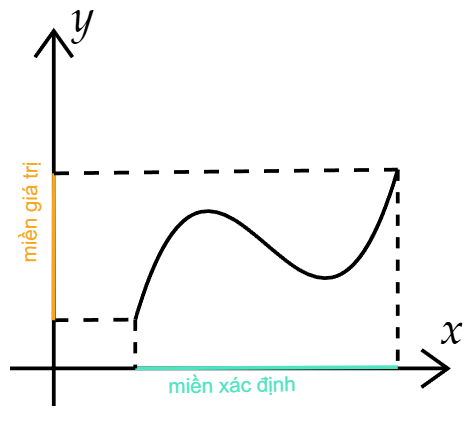
\includegraphics[width= 0.8\linewidth]{Tuan1/ảnh/hamso1.png}
        \caption{}
    \end{subfigure}
    \hfill
    \begin{subfigure}{0.4\textwidth}
        \centering
        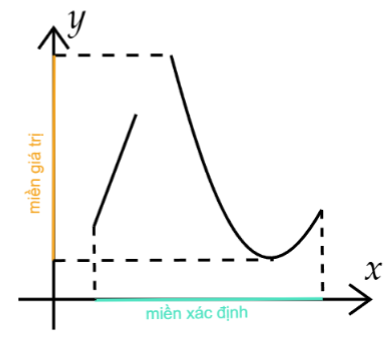
\includegraphics[width=0.8\linewidth]{Tuan1/ảnh/hamso2.png}
        \caption{}
    \end{subfigure}
    \caption{Ví dụ về đồ thị hàm số}\label{anh1.2}
    \end{figure}

Các điểm này có thể là vô số, tạo thành những đường cong hoặc đường thẳng trên mặt phẳng, liên tục hoặc rời rạc. Song không phải mọi đường bất kỳ đều là đồ thị của một hàm số nào đó. Để là đồ thị của một hàm số, mỗi hoành độ $x$ phải tương ứng với một tung độ $y$ duy nhất. Nghĩa là không được có hai điểm khác nhau trên đồ thị có cùng hoành độ nhưng khác tung độ.

Một cách trực quan,\emph{ không có đường thẳng thẳng đứng (vuông góc với trục hoành) nào cắt đồ thị của một hàm số nhiều hơn một lần.} (xem \ref{anh1.2})
\begin{figure}[htbp]
    \centering
    \begin{subfigure}{0.4\textwidth}
        \centering
        \includegraphics[width= 7cm, height=6cm]{Tuan1/ảnh/hamsochuan.png}
        \caption{Đồ thị hàm số}
    \end{subfigure}
    \hfill
    \begin{subfigure}{0.4\textwidth}
        \centering
        \includegraphics[width=7cm, height=6cm]{Tuan1/ảnh/khongphaihamso.png}
        \caption{Không phải đồ thị hàm số}
    \end{subfigure}
    \caption{So sánh}\label{anh1.3}
    \end{figure}

%%%Các hàm
\subsection{Các hàm thông dụng}

Trong khi xử lý các bài toán, chúng ta thường gặp các hàm số có dạng tổng quát. Các hàm này được phân loại theo dạng biểu thức của chúng. Dưới đây là một số loại hàm số cơ bản:   \begin{itemize}
    \item Hàm \emph{tuyến tính} có dạng $f(x) = ax + b$, với $a$ và $b$ là các hằng số. Đồ thị của hàm tuyến tính là một đường thẳng.\newline Ví dụ: $ 2x+3$.
    \item Hàm \emph{đa thức} có dạng $P(x) = a_n x^n + a_{n-1} x^{n-1} + \ldots + a_1 x + a_0$, với $a_n, a_{n-1}, \ldots, a_0$ là các hằng số và $n\in\mathbb{N}$ là bậc của đa thức.\newline Ví dụ: $x^2 - 4x + 4; x^5 + 2x^2 - 5x + 1$; $3x+2$.
    \item Hàm \emph{luỹ thừa} có dạng $f(x)=x^\alpha$, với $\alpha\in\mathbb{R}$ là một hằng số.\newline Ví dụ: $x^2, x^{-3}=\frac{3}{x}, x^{5/2}=\sqrt{x^5}=(\sqrt x)^5$.     
    \item Hàm tỷ lệ có dạng $f(x) = \frac{P(x)}{Q(x)}$, với $P(x)$ và $Q(x)$ là các đa thức. Ví dụ: $\frac{x^2+1}{x-2}$.    
\end{itemize}
Trên đây được gọi chung là các hàm \emph{đại số}, tức là các hàm có thể được biểu diễn bằng các toán tử đại số như cộng, trừ, nhân, chia và lũy thừa.\newline
Ví dụ : $\frac{\left(x^5+x^3-x^2+4\right)^{3/2}}{x+\sqrt x}$.
\vspace{8pt}

Ta cũng liệt kê thêm một số hàm không thuộc loại trên.\newline
Ví dụ như các hàm \emph{siêu việt}:\begin{itemize}
    \item Hàm \emph{lượng giác} là các hàm $\sin x,\cos x, \tan x, \dots$ mà có thể được định nghĩa thông qua các điểm trên một đường tròn đơn vị.
    \item Hàm \emph{mũ} và \emph{lôgarit} lần lượt có dạng $f(x) = a^x$ và $f(x) = \log_a x$, với $a > 0$ là một hằng số. Cái sau là hàm \emph{nghịch đảo} của cái trước, tức là $\log_a a^x = x$ và $a^{\log_a x} = x$.\newline Ví dụ: $2^x \text{ và } \log_2 x$; $e^x \text{ và } \ln x$.
\end{itemize}
Hay, hàm xác định từng phần là các hàm được xác định bởi các công thức khác nhau trên các miền khác nhau của tập xác định.\newline
Ví dụ, hàm giá trị tuyệt đối $f(x) = |x|$ được định nghĩa:
\begin{equation*}
    f(x) = \left\{
\begin{aligned}
x  & \quad \text{nếu } x \geq 0 \\
-x   & \quad \text{nếu } x < 0
\end{aligned}
\right\}.
\end{equation*}

Trong tất cả những hàm vừa liệt kê lại có một số hàm có tính chất chung. Chẳng hạn như tính chẵn lẻ, tính đồng biến nghịch biến, tính liên tục,...\newline
Trước khi sang phần tiếp theo, hãy nói qua thêm một khái niệm nữa, đó là \emph{hàm hợp}. Ta biết rằng hàm số là một thứ mà ta cho vào một giá trị và sẽ cho ra một giá trị nào đó. Trên cơ sở này, hàm hợp là một hàm số mà đầu vào của nó là đầu ra của một hàm số khác.\newline
Xét hai hàm $f(x)$ và $g(x)$, hàm hợp của chúng được ký hiệu là $f(g(x))$ và được đọc là "hàm $f$ của hàm $g$ tại $x$". Hàm hợp này sẽ nhận đầu vào là giá trị của hàm $g(x)$ và trả về giá trị của hàm $f$ tại điểm đó.\newline    
Ví dụ: $f(x)=x^2$, $g(x)=\sin x$ vậy $f(g(x))=f(\sin x)=\sin^2 x$.

\section{Giới Hạn Hàm Số}
\subsection{Một ví dụ về giới hạn}
Xét hàm số $y=x^2$, phóng to đồ thị vào gần điểm $(1;1)$:
\begin{figure}[h!]
    \centering
    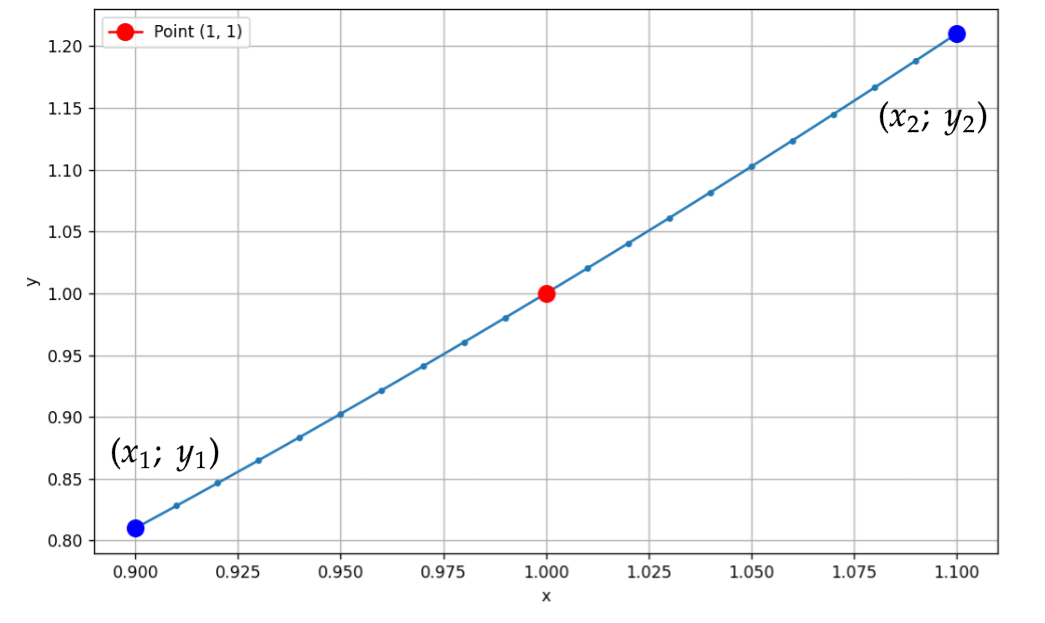
\includegraphics[width=0.6\textwidth]{Tuan1/ảnh/0.9-1.1.png}
    \caption{Đồ thị \(y=x^2\) được phóng to trong khoảng $[0.9;1.1]$}
    \label{anh3}
\end{figure}

Hãy tưởng tượng có hai con bọ xuất phát từ hai điểm xanh và bò lại \emph{gần} điểm màu đỏ trên con đường tạo thành từ đoạn đồ thị này. Để tiến tới đó, con bọ thứ nhất, xuất phát từ bên trái, phải đi qua các điểm nằm trong khoảng $[0.9;0.999]$. Trong khi đó, con bọ thứ hai, xuất phát từ bên phải, phải trải qua các điểm nằm trong khoảng $[1.001;1.1]$.

Ta thấy chúng quả thực đang tiến tới \emph{gần} điểm $(1;1)$ bởi không chỉ hoành độ mà tung độ của chúng cũng dần tiến đến giá trị bằng $1$ (như được kiểm chứng trong bảng bên dưới).
\begin{table}[H]
    \centering
    \caption{Bảng giá trị \( y = x^2 \) khi \( x \text{~tới gần } 1 \)}
    \begin{tabular}{|c|c||c|c|}
    \hline
    \multicolumn{2}{|c||}{Bên trái} & \multicolumn{2}{c|}{Bên phải} \\
    \hline
    \( x \) & \( y \) & \( x \) & \( y \) \\
    \hline
    0.900 & 0.8100 & 1.100 & 1.2100 \\
    0.925 & 0.8556 & 1.075 & 1.1556 \\
    0.950 & 0.9025 & 1.050 & 1.1025 \\
    0.975 & 0.9506 & 1.025 & 1.0506 \\
    0.990 & 0.9801 & 1.010 & 1.0201 \\
    0.995 & 0.9900 & 1.005 & 1.0100 \\
    0.999 & 0.9980 & 1.001 & 1.0020 \\
    \hline
    \end{tabular}
\end{table}
   
Sau khi cả hai lần lượt tới điểm $(0.999;0.9980)$ và $(1.001;1.0020)$, chúng tiếp tục di chuyển và để quan sát quá trình tiếp theo, ta tiếp tục phóng to khoảng đồ thị nằm giữa chúng:
\begin{figure}[h!]
    \centering
    \includegraphics[width=0.6\textwidth]{Tuan1/ảnh/0.999.png}
    \caption{Khoảng \([0.999;1.001]\) với hai vị trí ban đầu mới được đánh dấu }
\end{figure}

Như vậy sự phóng to này có thể tiếp tục vô hạn lần nữa trong khi khoảng cách giữa hai con bọ và điểm màu đỏ càng nhỏ dần. Dù vậy, ta biết rằng trong thực tế rồi chúng sẽ đến được điểm màu đỏ.\footnote{Đoạn đường mà chúng trải qua sẽ nhỏ dần. Quãng đường chúng phải đi sẽ là một tổng có vô số hạng tử với các hạng tử phía sau ngày càng nhỏ mà may thay, tổng này có giá trị hữu hạn. }\newline
Nhưng nếu giả sử tại hai điểm nào đó rất rất gần $(1;1)$, đường bị gãy (và phía dưới chúng là vực sâu), hai chú bọ không thể tiến lên được nữa. Rồi vấn đề tiếp tục xảy đến rằng chỉ cần vị trí của các điểm này \emph{luôn gần điểm $(1;1)$ hơn chúng}, hai chú bọ đáng thương sẽ phải tiếp tục di chuyển với một quá trình "phóng to vô hạn" như vậy mãi mãi.

\begin{definition}
    Giả sử $f(x)$ xác định trong một khoảng (miền) giá trị nào đó của $x$ có chứa $a$ (có thể xác định hoặc không xác định tại $a$). Khi đó ta viết
    \begin{equation*}\lim_{x\rightarrow a}f(x)=L\end{equation*}
và nói\qquad\qquad\qquad "giới hạn của $f(x)$, khi $x$ tiến tới $a$, bằng $L$"\newline nếu chúng ta có thể lấy các giá trị $f(x)$ gần $L$ một cách tuỳ ý bằng cách lấy các giá trị của $x$ đủ gần $a$ (từ bất cứ phía nào), nhưng không được bằng $a$.
\end{definition}

Định nghĩa vừa đưa ra về giới hạn có vẻ khá trừu tượng và thiếu chặt chẽ. Dẫu thế trong khuôn khổ phần này, ta sẽ không đào sâu vào vấn đề chặt chẽ trong lí luận giới hạn. Thay vào đó, hy vọng với ví dụ vừa rồi, các bạn có thể phần nào thu được trực giác về khái niệm này.\newline

\begin{definition}
    Ta viết \begin{equation*}\lim_{x\rightarrow a^-}f(x)=L\end{equation*}
để nói rằng giới hạn của $f(x)$ khi $x$ tiến tới $a$ từ phía bên trái (tức là $x$ nhỏ hơn $a$) bằng $L$. 
\end{definition}

Tương tự, với $x>a$, ta viết $$\lim_{x\rightarrow a^+}f(x)=L .$$ 
\begin{theorem}
    \begin{equation*}\lim_{x\rightarrow a}f(x)=L \leftrightarrow \lim_{x\rightarrow a^-}f(x)=L, \lim_{x\rightarrow a^-}f(x)=L.\end{equation*}   
\end{theorem}

Nghĩa là nếu giới hạn trái và phái khi $x\rightarrow a$ cùng bằng nhau thì giới hạn của hàm số tại điểm đó là tồn tại.
Ta cũng thừa nhận nếu hàm số tồn tại giới hạn tại điểm nào đó, giới hạn đó là duy nhất. Như đã thể hiện thông qua ví dụ ở trên.

\subsection{Giới hạn ở vô cùng và một số quy tắc tính giới hạn}
\begin{definition} Ta viết
    \begin{equation*}\lim_{x\rightarrow a}f(x)=\infty\end{equation*}
nếu f(x) có thể nhận các giá trị lớn tuỳ ý khi cho $x$ nhận các giá trị đủ gần $a$, nhưng không được bằng $a$.
\end{definition}
Điều này dễ hiểu nếu xét hàm $1/x$ với $a=0$ : lấy 1 chia 100, rồi lấy 1 chia $10$, chia $0.1$, $0.01,...$ kết quả thu được sẽ ngày càng lớn. Nếu lấy 1 chia $1/10^6$, sẽ có được $10^6$. Và cứ thế.
Chú ý rằng vô hạn không phải một con số. Nó, ở đây, là một giới hạn.\newline
Ta cũng có thể có điều ngược lại:$$\lim_{x\rightarrow\infty}f(x)=L$$ để diễn tả khi $x$ nhận các giá trị lớn tuỳ ý (tiến tới vô cùng) thì $f(x)$ tiến tới gần giá trị xác định $L$ một cách tuỳ ý. Trong trường hợp hàm số là 1/$x$, ý của ta là tương đương với cho $x$ nhận một giá trị nào đó đủ lớn ($10^2,10^3,10^4,10^n...$) sao cho có thể coi $1/x =10^{-n}\approx 0.$ 

Cũng có thể viết  $$\lim_{x\rightarrow\infty}f(x)=\infty.$$ để nói rằng $f(x)$ có thể nhận các giá trị lớn tuỳ ý khi $x$ đủ lớn.\newline    
\vspace{5pt}

 Giả sử $c$ và $d$ là các hằng số, \[\lim_{x\rightarrow a}f(x)=A \text{ và } \lim_{x\rightarrow a}g(x)=B, \] ta thừa nhận những tính chất và quy tắc sau:
\begin{itemize}
 \item \emph{Tính chất tuyến tính:} \[\lim_{x\rightarrow a}(cf(x)\pm dg(x))=cA \pm dB.\]
 \item \emph{Tính duy nhất:} \[\text{Nếu } f(x)=g(x)~khi~x\neq a,\text{thì } A=B.\]
 \item \emph{Quy tắc nhân:} \[\lim_{x\rightarrow a}f(x)g(x)=AB.\]
 \item \emph{Quy tắc chia:} \[\lim_{x\rightarrow a}f(x)/g(x)=A/B, B\neq 0.\]
 \item \emph{Quy tắc luỹ thừa:} \[\lim_{x\rightarrow a}(f(x))^{m/n}=A^{m/n}.\]
\end{itemize}
\begin{theorem}{Định lý kẹp}
    Xét các hàm só $g(x), f(x), h(x)$ xác định trên miền chứa $a$ (có thể có hoặc không xác định tại $a$), với mọi $x$ khác $a$:
    \[g(x)\leq f(x)\leq h(x),\] và giả sử \[\lim_{x\rightarrow a}g(x)=\lim_{x\rightarrow a}h(x)=L.\]
    Thì, \[\lim_{x\rightarrow a}f(x)=L.\]
\end{theorem}
\section{Đạo Hàm}
\subsection{Khái niệm}
\begin{definition}
\textbf{Đạo hàm} của hàm số $f$ tại giá trị $a$, kí hiệu bởi $f'(a)$, là
    \begin{equation}
        f'(a)=\lim_{\Delta x\rightarrow 0}\frac{f(a+\Delta x)-f(a)}{\Delta x}
    \end{equation}
nếu giới hạn này tồn tại.
\end{definition}

Ý nghĩa hình học trực quan của đạo hàm là nó thể hiện độ dốc của đồ thị và tốc độ biến thiên của hàm số. Ta xét độ dốc của các đường cát tuyến đi qua A:\footnote{Ở đây góc $\theta_M$ và $\theta_N$ có giá trị âm.}
\begin{figure}[H]
\centering 
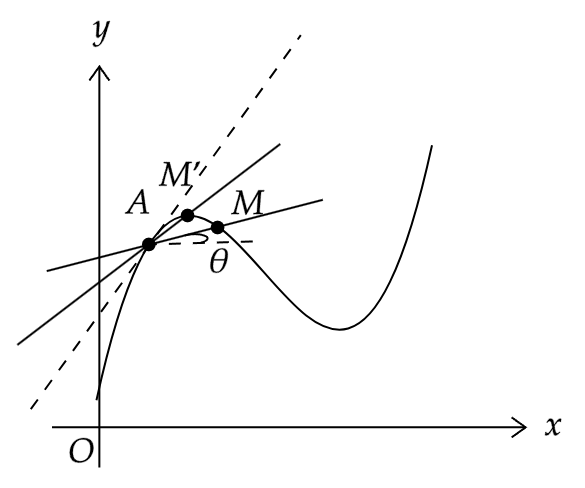
\includegraphics[width=1\textwidth]{Tuan1/ảnh/cattuyen.png}
\caption{Độ dốc của các đường cát tuyến đi qua A (các góc $\theta_M$, $\theta_N$, $\theta_P$)}
\end{figure}

Nếu các điểm $M$, $N$, $P$ tiến gần đến điểm $A$, độ dốc của các đường cát tuyến này sẽ tiến gần đến một giá trị nhất định, chính là độ dốc của tiếp tuyến. Độ dốc này chính là đạo hàm của hàm số tại điểm $A$:
\begin{figure}[H]
\centering
\includegraphics[width=1\textwidth]{Tuan1/ảnh/tocdobienthien.png}
\caption{Liên hệ giữa đạo hàm và độ dốc (độ lớn góc $\theta$) của đồ thị}
\end{figure}

Cũng từ hình vẽ trên, ta có thể thấy đạo hàm chính là hệ số góc của tiếp tuyến đồ thị. Vì thế, ta có thể biểu diễn phương trình của đường tiếp tuyến tại $x=a$:
\begin{equation}
    y=f(a)+f'(a)(x-a)
\end{equation}



\subsection{Một số quy tắc đạo hàm}
Dưới đây là đạo hàm của một số hàm thông dung:

\begin{itemize}
\item\textit{Đạo hàm của hàm đa thức}:
\begin{equation}
    \frac{d}{dx}x^n=nx^{n-1}
\end{equation}
\item\textit{Đạo hàm của các hàm lượng giác}:
\begin{center}
\begin{tabular}{cc}
\(
\begin{aligned}
    &\dfrac{d}{dx}(\sin x)=\cos x\\
    &\dfrac{d}{dx}(\cos x)=-\sin x
\end{aligned}
\)
&
\(
\begin{aligned}
    &\dfrac{d}{dx}(\tan x)=\sec^2 x\\
    &\dfrac{d}{dx}(\cot x)=-\csc^2 x
\end{aligned}
\)
\end{tabular}
\end{center}
\item\textit{Đạo hàm của hàm mũ và hàm logarit}:
\begin{equation}
    \frac{d}{dx}e^x=e^x,\quad \frac{d}{dx}\ln x=\frac{1}{x}
\end{equation}
\end{itemize}

Tương tự như giới hạn, đạo hàm cũng có một số tính chất quan trọng:
\begin{itemize}
    \item \textit{Tính chất tuyến tính}: Nếu $f(x)$ và $g(x)$ là hai hàm số theo $x$, và $c$ là một hằng số, thì
    \begin{equation}
        (cf+g)'=cf'+g'
    \end{equation}
    \item \textit{Quy tắc nhân}: Nếu $f(x)$ và $g(x)$ là hai hàm số theo $x$, thì
    \begin{equation}
        (fg)'=fg'+f'g
    \end{equation}
    \item \textit{Quy tắc chia}: Nếu $f(x)$ và $g(x)$ là hai hàm số theo $x$, với $g(x)\neq 0$, thì
    \begin{equation}
        \left(\frac{f}{g}\right)'=\frac{f'g-fg'}{g^2}
    \end{equation}
\end{itemize}
\subsection{Xấp xỉ tuyến tính và vi phân}
Tiếp theo ta sẽ nói về một ứng dụng quan trọng khác của đạo hàm. Nếu phóng to đồ thị tại điểm $x=a$, ta có thể thấy đồ thị hàm số trông khá gần với tiếp tuyến của nó tại điểm này.
\begin{figure}[H]
\centering
\includegraphics[width=1\textwidth]{Tuan1/ảnh/xapxituyentinh.png}
\caption{Phóng to đồ thị hàm số tại điểm $x=a$}
\end{figure}
Từ quan sát trên, ta có thể nghĩ tới một phép xấp xỉ.

\begin{definition}
    Ở lân cận điểm $x=a$, ta có thể xấp xỉ hàm số $f(x)$ bằng phương trình đường tiếp tuyến tại điểm này:
\begin{equation}
        f(x)\approx f(a)+f'(a)(x-a)
    \end{equation}
đây được gọi là \textbf{xấp xỉ tuyến tính}.
\end{definition}
Ý tưởng đằng sau phép xấp xỉ tuyến tính đôi khi được phát biểu bằng \textbf{phép lấy vi phân}.

\begin{definition}
    Nếu $y=f(x)$, \textbf{vi phân} $dx$ là một biến độc lập. Lúc đó \textbf{vi phân} $dy$ được xác định theo $dx$ bởi phương trình:
\begin{equation}
    dy=f'(x)dx
\end{equation}
\end{definition}
và \textbf{phép lấy vi phân} trên có ý nghĩa hình học như hình vẽ:

\begin{figure}[H]
\centering
\includegraphics[width=1\textwidth]{Tuan1/ảnh/viphan.png}
\caption{Ý nghĩa hình học của phép lấy vi phân}
\end{figure}
Từ kí hiệu bên trên, ta có thể viết lại đạo hàm theo cách khác:
\begin{equation}
    f'(x)=\frac{dy}{dx} 
\end{equation}
Đây được gọi là \textbf{kí hiệu Leibniz cho đạo hàm}.
\subsection{Quy tắc đạo hàm hợp}

Đối với một hàm số \(f(x)\) có dạng phức tạp theo \(x\), ta có thể viết lại nó dưới dạng hàm hợp \(f(g(x))\) sao cho \(f(g)\) và \(g(x)\) có dạng đơn giản hơn, sau đó áp dụng quy tắc sau để thực hiện phép đạo hàm:
\begin{theorem}
\textbf{Quy tắc đạo hàm hợp}: Nếu \(f\) là hàm số có đạo hàm tại \(g(x)\), và \(g\) là hàm số có đạo hàm tại \(x\), thì đạo hàm của hàm hợp \(f(g(x))\) được tính theo công thức:
\begin{equation}
    f'(x)=\frac{df}{dx}=\frac{df}{dg}\cdot\frac{dg}{dx}=f'(g(x))\cdot g'(x)
\end{equation}
\end{theorem}
\textit{Ví dụ: \(f(x)=\sqrt{x^2+1}\) có thể được viết lại dưới dạng hàm hợp \(f(g(x))\) với \(g(x)=x^2+1\).}

\textbf{Lưu ý:} Quy tắc đạo hàm hợp không đơn giản chỉ là khử đi tử và mẫu số giống như phép nhân phân số vì ý nghĩa của kí hiệu Leibniz không hoàn toàn giống với phân số thông thường. Việc chứng minh quy tắc này sẽ phức tạp hơn và sẽ là nhiệm vụ của bạn trong bài tập ....

\subsection{Về tính toán số}
Giả sử ta muốn tính đạo hàm của \(y(x)\) bằng các công cụ lập trình, sẽ là tự nhiên nếu sử dụng trục tiếp định nghĩa của đạo hàm:
\[y(x_0+\epsilon)\approx y(x_0)+\epsilon y'(x_0).\] Ở đây \(\epsilon\) là một con số rất nhỏ, ví dụ như \(0.01\), hay nếu cần chính xác hơn, có thể là \(0.001\),v.v. Như vậy, việc ta cần làm chỉ là khai báo hàm \(y(x)\) rồi chọn một bước nhảy thích hợp. Ta có thể làm điều tương tự đối với các đạo hàm cấp cao hơn: \[y'(x_0 +\epsilon)\approx y'(x_0)+\epsilon y''(x_0).\]

\section{Ứng Dụng Của Đạo Hàm Và Vi Phân}
\subsection{Giá trị cực đại và cực tiểu}
Đạo hàm có một ứng dụng quan trọng trong việc xác định các \textbf{cực đại địa phương} và \textbf{cực tiểu địa phương}. Trước hết, ta sẽ tìm hiểu về hai khái niệm này.
\begin{definition}
    \textbf{Cực đại địa phương} của hàm số \(f(x)\) tại điểm \(x=a\) là giá trị \(f(a)\) nếu tồn tại một khoảng mở \((a-\delta, a+\delta)\) với \(\delta > 0\) sao cho:
    \[
    f(a) \geq f(x) \quad \forall x \in (a-\delta, a+\delta)
    \]
\end{definition}
\begin{definition}
    \textbf{Cực tiểu địa phương} của hàm số \(f(x)\) tại điểm \(x=a\) là giá trị \(f(a)\) nếu tồn tại một khoảng mở \((a-\delta, a+\delta)\) với \(\delta > 0\) sao cho:
    \[
    f(a) \leq f(x) \quad \forall x \in (a-\delta, a+\delta)
    \]
\end{definition}
Và các điểm trên được gọi chung là \textbf{cực trị} của hàm số \(f(x)\).
\begin{figure}[H]
\centering
\includegraphics[width=0.8\textwidth]{Tuan1/ảnh/cuctri.png}
\caption{Cực đại địa phương (điểm \(M\)) và cực tiểu địa phương (điểm \(N\))}
\end{figure}
Từ hình vẽ trên, ta có thể thấy tại các điểm cực trị, tiếp tuyến của đồ thị nằm ngang. Từ đó, ta có định lý sau:
\begin{theorem}
    \textbf{Định lý Fermat}: Nếu hàm số \(f\) có cực trị tại \(a\), thì \(f'(a)=0\) nếu đạo hàm này tồn tại.
\end{theorem}
Tuy nhiên, định lý đảo của định lý trên không đúng.
\begin{figure}[H]
\centering
\includegraphics[width=0.8\textwidth]{Tuan1/ảnh/khongcuctri.png}
\caption{Điểm uốn \(A\) của đồ thị hàm số}
\end{figure}
Từ hình vẽ trên, ta có thể thấy đạo hàm của hàm số tại điểm \(A\) bằng 0 nhưng đây không phải là điểm cực trị. Điểm này được gọi là \textbf{điểm uốn} của đồ thị hàm số.

Một cách để xác định điểm cực trị là cực đại hay cực tiểu địa phương là sử dụng định lý sau:
\begin{theorem}
    Xét hàm \(f\) có đạo hàm bằng 0 tại điểm \(a\), nếu:
    \begin{itemize}
    \item \(f''(a) > 0\), thì \(f(a)\) là cực tiểu địa phương.
    \item \(f''(a) < 0\), thì \(f(a)\) là cực đại địa phương.
    \end{itemize}
\end{theorem}
Nếu \(f''(a) = 0\), ta không thể kết luận được gì về điểm này. Trong trường hợp đó, ta sẽ cần sử dụng các phương pháp sẽ được bàn luận trong các bài tập...

\subsection{Định lý giá trị trung bình}
Định lý giá trị trung bình là một trong những định lý quan trọng của giải tích. Nhưng trước khi đến với định lý này, ta sẽ cần giới thiệu một định lý khác:
\begin{theorem}
\textbf{Định lý Rolle}: Nếu hàm số \(f\) là liên tục và khả vi trên khoảng \([a, b]\), và \(f(a) = f(b)\), thì tồn tại ít nhất một điểm \(c \in (a, b)\) sao cho \(f'(c) = 0\).
\end{theorem}
Chúng ta có thể nhìn vào đồ thị của các hàm số thỏa mãn điều kiện trên để thấy được ý nghĩa trực quan của điểm \(c\):
\begin{figure}[H]
\centering
\includegraphics[width=0.8\textwidth]{Tuan1/ảnh/ĐL Rolle.png}
\caption{Định lý Rolle}
\end{figure}
Việc chứng minh chặt chẽ sẽ là nhiệm vụ của bạn trong bài tập....

Định lý giá trị trung bình là một mở rộng của định lý Rolle. Định lý này phát biểu như sau:
\begin{theorem}
\textbf{Định lý giá trị trung bình}: Nếu hàm số \(f\) là liên tục và khả vi trên khoảng \([a, b]\), thì tồn tại ít nhất một điểm \(c \in (a, b)\) sao cho:
\begin{equation}
f'(c)=\frac{f(b) - f(a)}{b - a}
\end{equation}
hay
\begin{equation}
f(b) - f(a) = f'(c)(b - a)
\end{equation}
\end{theorem}
Khi này, độ dốc của tiếp tuyến tại điểm \(c\) bằng với độ dốc của cát tuyến nối giữa hai điểm \(a\) và \(b\):
\begin{figure}[H]
\centering
\includegraphics[width=0.8\textwidth]{Tuan1/ảnh/ĐL GTTB.png}
\caption{Định lý giá trị trung bình}
\end{figure}
Chứng minh định lý này sẽ là nhiệm vụ của bạn trong bài tập....
\subsection{Xấp xỉ đa thức của hàm số}
Trong thực tế, chúng ta thường cần tính giá trị của một hàm số tại một điểm nào đó. Tuy nhiên, việc tính toán trực tiếp có thể phức tạp hoặc không khả thi. Do đó, chúng ta thường sử dụng các đa thức xấp xỉ để ước lượng giá trị của hàm số.
\begin{theorem}\label{thm:taylor}
Nếu \(f\) có một khai triển bằng chuỗi lũy thừa tại \(a\), tức là nếu
\begin{equation}
f(x)=\sum_{n=0}^{\infty}c_n(x-a)^n
\end{equation}
thì các hệ số của nó được cho bởi công thức sau
\begin{equation}
c_n=\frac{f^{(n)}(a)}{n!}
\end{equation}
trong đó \(f^{(n)}(a)\) là đạo hàm bậc \(n\) của hàm số \(f\) tại điểm \(a\).

Chuỗi lũy thừa này được gọi là \textbf{chuỗi Taylor} của hàm số \(f\) tại điểm \(a\).
\end{theorem}
Khi ta chỉ lấy một vài số hạng của chuỗi, ta thu được một phép xấp xỉ:
\begin{definition}
\textbf{Khai triển Taylor bậc \(n\)} của hàm số \(f\) tại điểm \(a\):
\begin{equation}
f(x)\approx f(a)+f'(a)(x-a)+\frac{f''(a)}{2!}(x-a)^2+\cdots+\frac{f^{(n)}(a)}{n!}(x-a)^n
\end{equation}
\end{definition}
Càng lấy tới bậc càng cao, độ chính xác của phép xấp xỉ càng cao.
\section{Phương Trình Tham Số}
\input{Tuan1/phuongtrinhthamso.tex}
\section{Hướng Dẫn Học}
\section{Bài tập}
\subsection*{Hàm số}
\textbf{Bài 1.1:} Tìm miền xác định của các hàm số sau
\begin{enumerate}[label=(\alph*)]
\item \(\frac{x-2}{2x-1}\)
\item $\frac{\ln(1+x)}{x-1}$
\item $\sqrt{1-2x}+3\arcsin\left(\frac{3x-1}{2}\right)$ \quad ($\sin{x}=y\leftrightarrow x=\arcsin y$)
\item $\frac{1}{x e^x}$
\item $\ln{(3x+1)}+2\ln{(x+1)}$
\end{enumerate}

\vspace{5pt}
\textbf{Bài 1.2:} Tìm tập hợp giá trị của các hàm số sau
\begin{enumerate}[label=(\alph*)]
\item $x^2 -6x+5$
\item $2+3\sin x$
\item $|x| + x + 1 = y + |y|$
\item $4^{-x^2}$
\end{enumerate}
\vspace{5pt}

\textbf{Bài 1.3:} Chứng minh
\begin{enumerate}[label=(\alph*)]
\item $\sin(\alpha+\beta)=\sin\alpha\cos\beta + \sin\beta\cos\alpha.$
\item $\cos(\alpha+\beta)=\cos\alpha\cos\beta - \sin\alpha\sin\beta.$
\end{enumerate}

\emph{Gợi ý:} \href{https://vi.wikipedia.org/wiki/%C4%90%E1%BB%8Bnh_l%C3%BD_Ptoleme}{Định lý Ptoleme}

\subsection*{Vẽ đồ thị của hàm}
\emph{Chú ý}: Ta có thể vẽ đồ thị của hàm có dạng $y=Af(k(x-a))+b$ theo đồ thị của hàm $f(x)$
\begin{itemize}
    \item $y=f(x-a)$: đồ thị ban đầu được tịnh tiến theo trục $Ox$ một đại lượng $a$.
    \item $y=f(x)+b$: đồ thị ban đầu được tịnh tiến theo trục $Oy$ một đại lượng $b$.
    \item $y=Af(x)$: đồ thị xuất phát được giãn ra $A$ lần theo trục $Oy$.
    \item $y=f(kx)$: đồ thị xuất phát được giãn ra $1/k$ lần theo trục $Ox$.
\end{itemize}
\textbf{Bài 1.4:} Vẽ đồ thị các hàm số trong hai bài tập ở trên bằng

a. Desmos 
\vspace{5pt}

b. Python (đối với hàm tuần hoàn thì vẽ trong khoảng $[-\pi;\pi]$; đối với các hàm khác, lựa chọn điểm đầu và cuối sao cho thu được mọi miền của hàm)
\vspace{5pt}

\textbf{Bài 1.5}: Vẽ một hình tam/tứ/ngũ/lục giác đều bằng Desmos và Python.
\vspace{5pt}

\textbf{Bài 1.6:} Giải các phương trình sau thông qua việc vẽ đồ thị bằng Python
\begin{enumerate}[label=(\alph*)]
    \item $\tan x= x.$
    \item $\ln x = x-2.$
    \item $x^3 -15x =4.$
    \item $x^5 -4x^2 +3=0.$
\end{enumerate}
\subsection*{Hàm hợp}

\textbf{Bài 1.7:} Các hàm số trong \textbf{Bài 1.1} là hàm hợp của những hàm nào? Hãy phân tích cụ thể thứ tự của chúng.
\vspace{5pt}

\textbf{Bài 1.8:} Nguyên lý quy nạp\newline

Cho $S_n$ là một phát biểu về số nguyên dương $n$. Giả sử rằng:
\begin{itemize}
    \item $S_1$ đúng.
    \item $S_{k+1}$ đúng khi $S_k$ đúng.
\end{itemize}
Khi đó $S_n$ đúng với tất cả các số nguyên dương $n$.\newline
Sử dụng điều này để giải các bài toán sau:
\begin{enumerate}[label=(\alph*)]
    \item Nếu $f_0(x) =x/(x+1)$ và $f_{n+1}(x)=f_0(f_n(x))$ với $n=0, 1, 2,\dots$, tìm một công thức cho $f_n(x)$.
\item Nếu $f_0(x) =x^2$ và $f_{n+1}(x)=f_0(f_n(x))$ với $n=0, 1, 2,\dots$, tìm một công thức cho $f_n(x)$.
\end{enumerate}
\vspace{5pt}
\subsection*{Phương trình hàm}
\textbf{Bài 1.9:} Tìm hàm \(f: \mathbb{R}\rightarrow\mathbb{R}\) sao cho
\begin{enumerate}[label=(\alph*)]
    \item \(f(a+b)=f(a)+f(b)\)
    \item \(f(ab)=f(a)f(b)\)
    \item \(f(a+b)=f(a)f(b)\)
    \item \(f(ab)=f(a)+f(b)\)
\end{enumerate}

\subsection*{Giới hạn hàm số}
\textbf{Bài 1.10:} Chứng minh
\begin{enumerate}[label=(\alph*)]
    \item $$\lim_{x\rightarrow 0}\frac{\sin x}{x}=1.$$
    \item $$\lim_{x\rightarrow\infty}\left(1+\frac{1}{x}\right)^x =e=2,71828... .$$
    \item \[\lim_{x\rightarrow 0}\frac{(1+x)^m -1}{x}=m.\]
\end{enumerate}
và vẽ đồ thị tương ứng để kiểm tra lại.
\vspace{5pt}

\textbf{Bài 1.11:} Tính các giới hạn sau 
\begin{enumerate}[label=(\alph*)]
    \item $$\lim_{x\rightarrow 4}\frac{5x+2}{2x+3}$$
    \item $$\lim_{x\rightarrow \infty}\frac{3x+5}{2x+7} $$
    \item $$\lim_{x\rightarrow\infty}\frac{x^3 +2x^2 +3x+4}{4x^3 +3x^2 +2x+1}$$
    \item $$\lim_{x\rightarrow\infty}\frac{3x^4 -2}{\sqrt{x^8+3x+4}}$$
    \item \[\lim_{x\rightarrow\infty}\sqrt{x^2 +8x+3}-\sqrt{x^2+4x+3}\]
    \item \[\lim_{x\rightarrow 3}\frac{x^2 -9}{x^2-3x}\]
    \item \[\lim_{x\rightarrow 1}\frac{x^3 -x^2 -x+1}{x^3+x^2 -x-1}\]
    \item \[\lim_{x\rightarrow 2}\frac{\sqrt{1+x+x^2}-\sqrt{7+2x-x^2}}{x^2-2x}\]
\end{enumerate}
\vspace{5pt}

\textbf{Bài 1.12:} Sử dụng các kết quả trong \textbf{Bài 1.10} tính
\begin{enumerate}[label=(\alph*)]
    \item \[\lim_{x\rightarrow 0}\frac{\sin mx}{x}\]
    \item \[\lim_{x\rightarrow 0}\frac{1=\cos 5x}{x^2}\]
    \item \[\lim_{x\rightarrow\infty}\left(\frac{x^2+5x+4}{x^2-3x+7}\right)^x\]
    \item \[\lim_{x\rightarrow 2}\left(\frac{x}{2}\right)^{\frac{1}{x-2}}\]
\end{enumerate}

\subsection*{So sánh các vô cùng bé}
 Giả sử \(\alpha(x)\text{ và }\beta(x)\) là các vô cùng bé khi $x\rightarrow a$. Hay, \(\lim_{x\rightarrow a}\alpha(x)=0\) và \(\lim_{x\rightarrow a}\beta(x)=0\).
\begin{itemize}
    \item Nếu \(\lim_{x\rightarrow a}\frac{\alpha}{\beta}=0\), thì ta nói rằng $\alpha$ là vô cùng bé bậc cao so với $\beta$, kí hiệu $\alpha=o(\beta).$ 
    \item Nếu \(\lim_{x\rightarrow a}\frac{\alpha}{\beta}=m ( m\neq 0)\), thì ta nói \(\alpha\text{ và }\beta\) là các vô cùng bé cùng bậc. Đặc biệt nếu \(m=1\), ta gọi chúng là các vô cùng bé tương đương, kí hiệu $\alpha\sim \beta.$
    \item Nếu \(\alpha^k\) và \(\beta\) là các vô cùng bé cùng bậc, trong đó \(k>0\), ta nói rằng vô cùng bé \(\beta\) có bậc \(k\) so với \(\alpha\).
\end{itemize}
Ta chú ý một số tính chất của các đại lượng vô cùng bé:
\begin{itemize}
    \item Tích hai vô cùng bé là vô cùng bé cấp cao so với các nhân thức.
    \item Các vô cùng bé là tương đương khi và chỉ khi hiệu của chúng là vô cùng bé cấp cao so với chúng.
    \item Nếu tỷ số của hai vô cùng bé có giới hạn, thì giới hạn này không đổi nếu ta thay mỗi vô cùng bé bằng một vô cùng bé tương đương.
\end{itemize}
Lưu ý sự tương đương của các đại lượng vô cùng bé sau đây: nếu \(x\rightarrow 0\) thì \[\sin x\sim x, \tan x\sim x, \arcsin x\sim x, \arctan x\sim x, \ln(1+x)\sim x\]

\textbf{Bài 1.13:} 
Bằng cách thay tử và mẫu số bằng các vô cùng bé tương đương, tính 
\begin{enumerate}[label=(\alph*)]
    \item \[\lim_{x\rightarrow 0}\frac{\sqrt{1+2x}-1}{\tan 3x}\]
    \item \[\lim_{x\rightarrow 0}\frac{\ln \cos x}{\ln (1+x^2)}\]
    \item \[\lim_{x\rightarrow 0}\frac{(1+x)^{3/5}-1}{(1+x)(1+x)^{2/3}-1}\]
\end{enumerate}

\subsection*{Đạo hàm}
\textbf{Bài 1.14:} Chứng minh quy tắc đạo hàm hàm hợp.
\vspace{5pt}

\textbf{Bài 1.15:} Tính \(y'(x)\)
\begin{enumerate}[label=(\alph*)]
    \item \[y=\ln (x+\sqrt{x^2 +1}).\]
    \item \[y=\ln (\sqrt{2\sin x +1}+\sqrt{2\sin x -1}).\]
    \item \[y=\frac{x}{2}\sqrt{x^2 +k}+\frac{k}{2}\ln (x+\sqrt{x^2 +k}).\]
    \item \[y=\ln^2 \frac{\sqrt{4\tan x +1}-2\sqrt{\tan x}}{\sqrt{4\tan x +1}+2\sqrt{\tan x}}.\]
    \item \[y=\frac{1}{2}[(x+\alpha)\sqrt{x^2 +2\alpha x +\beta}+(\beta -\alpha^2)\ln(x+\alpha+\sqrt{x^2 +2\alpha x+\beta})].\]
    \item \[y=\sqrt{x+\sqrt{x+\sqrt{x}}}.\]
\end{enumerate}
Sau đó viết chương trình Python tính đạo hàm tại \(x=1\) để kiểm tra kết quả. 
\vspace{5pt}

\textbf{Bài 1.16:}
\begin{enumerate}[label=(\alph*)]
    \item Tìm góc giữa hai parabol \(y=8-x^2\) và \(y=x^2\).
    \item Tìm vận tốc tại thời điểm \(t_0 =4\mathrm{s}\) của điểm có quy luật chuyển động \(s(t)=4t-5t^2+12\).
\end{enumerate}

\subsection*{Phương pháp đạo hàm lấy lô-ga(tạm dịch)\footnote{Đọc thêm tại \href{https://en.wikipedia.org/wiki/Logarithmic_differentiation}{Logarithmic differentiation}}}
\textbf{Bài 1.17:} Tính 
\begin{enumerate}[label=(\alph*)]
    \item \[\frac{(2x-1)^3 \sqrt{3x+2}}{(5x+4)^2 \sqrt[3]{1-x}}.\]
    \item \[y=x^{x^2}.\]
\end{enumerate}
Hàm logarit nói chung và hàm \(\ln\) nói riêng đặc biệt có nhiều công dụng trong tính toán. Ta hãy liệt kê ra hai tính chất sẽ được bàn đến sau đây:
\begin{itemize}
    \item \(\ln(xy)=\ln x +\ln y \).
    \item \(\ln x^{\alpha} = \alpha \ln x\).
\end{itemize}
Tính chất đầu tiên là khả năng biến một tích thành một tổng, một thứ dễ tính hơn rất nhiều. Tính chất thứ hai lại có khả năng biến một hàm mũ phức tạp thành một tích rõ ràng hơn về sự phụ thuộc vào biến. \newline
Xét hàm \(y(x)\) có thể được viết thành tích của nhiều hàm số: \[y=f_{1}^{\alpha_1}(x).f_{2}^{\alpha_2}(x)\dots f_{n}^{\alpha_n}(x)\implies \ln y = \alpha_{1}\ln f_1 +\alpha_{2}\ln f_2 +\dots +\alpha_{n}\ln f_n.\]
Đạo hàm hai vế, \[\frac{y'}{y}=\alpha_{1} \frac{f'_1}{f_1}+\alpha_{2} \frac{f'_2}{f_2}+\dots +\alpha_{n} \frac{f'_n}{f_n}.\]
Hãy quay lại xử lý \textbf{Bài 1.15}  với công cụ này.
\vspace{5pt}

\textbf{Bài 1.18:} Tính 
\begin{enumerate}[label=(\alph*)]
  \item \[y=x^{\ln x}.\]  
  \item \[y=\frac{x^2 \sqrt{1+x}}{(x-1)^3 \sqrt[5]{5x-1}}.\]
\end{enumerate}

%%%%Đạo hàm và tích phân 1 chuỗi?-> Để sang tuần 3
\subsection*{Xấp xỉ tuyến tính}
\textbf{Bài 1.19:} Tính giá trị gần đúng của 
\begin{enumerate}[label=(\alph*)]
    \item $\sqrt[4]{15.8}$
    \item $\tan 46^\circ$
    \item Diện tích hình tròn bán kính $3.02\,\mathrm{m}$
    \item Thể tích hình cầu bán kính $2.01\,\mathrm{m}$. Biết thể tích hình cầu bán kính $R$ bằng $\frac{4}{3}\pi R^3$
\end{enumerate}
\vspace{5pt}

\textbf{Bài 1.20:} Tính \(\sqrt{e}\) chính xác đến \(0,0001\). 

\subsection*{Giá trị cực đại và giá trị cực tiểu}
\textbf{Bài 1.21:} Các điếm \(x=0\) của các hàm dưới đây là cực đại, cực tiểu hay điểm uốn?
\begin{enumerate}[label=(\alph*)]
    \item \(f(x)=1-3x^2+2x^4\)
    \item \(f(x)=x^3+x^5\)
    \item \(f(x)=x^6+2x^8-3x^{10}\)
\end{enumerate}

\textbf{Bài 1.22:} Chứng minh định lý Rolle.

\textbf{Bài 1.23:} Chứng minh định lý giá trị trung bình.

\textbf{Bài 1.24:} Chứng minh định lý 8.

\textbf{Bài 1.25:} Tìm chuỗi Taylor của các hàm sau tại điểm \(x=0\) (chuỗi Maclaurin):
\begin{enumerate}[label=(\alph*)]
    \item \(f(x)=\sin x\)
    \item \(f(x)=\cos x\)
    \item \(f(x)=e^x\)
    \item \(f(x)=\ln(1+x)\)
    \item \(f(x)=\sqrt{1+x}\)
\end{enumerate}

\section{Lời giải }
\textbf{Bài 1.1:}
\begin{enumerate}[label=(\alph*)]
    \item Hàm số xác định nếu \(2x-1\neq 0\), hay \(x\neq \frac{1}{2}\). Vì vậy \(X=(-\infty, 1/2)\cup (1/2,\infty)\).
    \item Hàm này xác định nếu \(x-1\neq 0\) và \(1+x>0\), hay \(x\neq 1\) và \(x>-1\). Vì vậy \(X=(-1,1)\cup (1,\infty)\).
    \item Số hạng thứ nhất nhận các giá trị thực khi \(x\leq\frac{1}{2}\). Số hạng thứ hai nhận các giá trị thực khi \(-1\leq\frac{3x-1}{2}\leq 1.\) Giải ra ta được \(x\leq 1, x\geq -\frac{1}{3}\). Do đó miền xác định là đoạn \([-1/3,1/2]\).
    \item Hàm số xác định với \(x\neq 0\). Nên \(X=(-\infty, 0)\cup(0,\infty)\).
    \item Điều kiện để hàm số xác định là \(3x+1\geq 0\) và \(x+1\geq 0\). Vậy \(X=[-1/3,\infty)\).
\end{enumerate}
\vspace{5pt}

\textbf{Bài 1.2:}
\begin{enumerate}[label=(\alph*)]
    \item Biến đổi, ta được \(f(x)=(x-3)^2 -4 \geq -4\). Do đó tập hợp giá trị của hàm là khoảng \(Y=[-4, \infty)\).
    \item Vì \(-1\leq \sin x\leq 1\), nên \(-3\leq\sin x\leq 3\). Do đó \(-1\leq f(x)\leq 5\) và \(Y=[-1, 5]\).
    \item Ta xem xét hai trường hợp : \(x<0 \text{ và } x>0\). \newline Nếu \(x<0\), \(y+\lvert y\rvert =1\). Giá trị của \(y\) không thể nhỏ hơn \(0\) vì điều này tương đương với \(y+\lvert y\rvert =0\). Do đó \(y=\frac{1}{2}\) trong trường hợp này.\newline Nếu \(x>0\), \(y\) chắc chắn lớn hơn \(0\) và do đó ta thu được hàm \(y=x+\frac{1}{2}\).\newline Dễ thấy, miền giá trị \(Y=[1/2,\infty)\).
    \item Miền giá trị của hàm là \(Y=[0,4]\).
\end{enumerate}
\vspace{5pt}

\textbf{Bài 1.3:}

Xét đường tròn tâm \(O\) có đường kính \(AC\) với độ dài bằng \(1\) và tứ giác \(ABCD\) nội tiếp đường tròn như hình bên.\raisebox{-0.2em}{\includegraphics[height=8 cm]{Tuan1/ảnh/unitcircle.png}}\newline
Vì \(\lvert AC\rvert =1\) nên tất cả độ dài trong biểu đồ được kết nối với sine hoặc cosine, và chú ý rằng hai góc ở đỉnh \(B\) và \(D\) là các góc vuông.\newline
Lúc này, theo định lý hàm sine trong tam giác, độ dài đoạn \(BD\) chính là \(\sin(\alpha+\beta)\). Định lý Ptoleme lại cho biết rằng \[\lvert AC\rvert \cdot\lvert BD\rvert =\lvert AB\rvert\dot\lvert CD\rvert +\lvert BC\rvert\dot\lvert AD\rvert.\]
và biểu thức này trở thành, sau khi ta thay các giá trị sine/cosine tương ứng:\[\sin(\alpha+\beta)=\sin\alpha\cos\beta +\sin\beta\cos\alpha.~(Q.E.D)\]
Sử dụng định lý Pythagoras, ta chứng minh được đẳng thức còn lại.

\vspace{5pt}
\textbf{Bài 1.10:}
\begin{enumerate}[label=(\alph*)]   
    \item Hàm số liên tục tại \(x=4\). Vậy nên \[\lim_{x\rightarrow 4}\frac{5x+2}{2x+3}=\frac{5\times 4+2}{2\times 4+3}=2.\]
    \item Ta thấy hàm số có dạng vô định \(\frac{\infty}{\infty}\) khi \(x\rightarrow\infty\). Một phương pháp điển hình để giải quyết tình huống này đó là chia bậc lớn nhất của \(x\) cho cả tử và mẫu, mà ở đây là bậc một. Khi đó, \[\lim_{x\rightarrow\infty}\frac{3x+5}{2x+7}=\lim_{x\rightarrow\infty}\frac{3+\frac{5}{x}}{2+\frac{7}{x}}=\frac{3}{2}.\] 
    \item Giới hạn của hàm số này cũng có dạng vô định \(\frac{\infty}{\infty}\). Tương tự, ta chia bậc lớn nhất của \(x\) cho cả tử và mẫu, mà ở đây là bậc ba. Khi đó, \[\lim_{x\rightarrow\infty}\frac{x^3 +2x^2 +3x+4}{4x^3 +3x^2 +2x+1}=\lim_{x\rightarrow\infty}\frac{1+\frac{2}{x}+\frac{3}{x^2}+\frac{4}{x^3}}{4+\frac{3}{x}+\frac{2}{x^2}+\frac{1}{x^3}}=\frac{1}{4}.\]
    \item Ta cũng có dạng vô định \(\frac{\infty}{\infty}\). Chia bậc lớn nhất  \(x^4\) cho cả tử và mẫu . Khi đó, \[\lim_{x\rightarrow\infty}\frac{3x^4 -2}{\sqrt{x^8+3x+4}}=\lim_{x\rightarrow\infty}\frac{3-\frac{2}{x^4}}{\sqrt{1+\frac{3}{x^7}+\frac{4}{x^8}}}=\frac{3}{1}=3.\]
    \item Ta có thể viết lại biểu thức này như sau: \[\lim_{x\rightarrow\infty}\sqrt{x^2 +8x+3}-\sqrt{x^2+4x+3}=\lim_{x\rightarrow\infty}\frac{(x^2 +8x+3)-(x^2+4x+3)}{\sqrt{x^2 +8x+3}+\sqrt{x^2+4x+3}}.\] Khi đó, chia bậc lớn nhất \(x\) cho cả tử và mẫu, và thu được, \[\lim_{x\rightarrow\infty}\frac{4}{\sqrt{1+\frac{8}{x}+\frac{3}{x^2}}+\sqrt{1+\frac{4}{x}+\frac{3}{x^2}}}=\lim_{x\rightarrow\infty}\frac{4}{2}=2.\]
    \item Giới hạn của hàm số này, nếu thay trực tiếp \(x=3\) sẽ có dạng vô định \(\frac{0}{0}\). Một phương pháp điển hình để giải quyết tình huống này, nếu có thể, là khử đi các nhân tử chung trong tử và mẫu. Dễ thấy, \[\lim_{x\rightarrow 3}\frac{x^2 -9}{x^2-3x}=\lim_{x\rightarrow 3}\frac{(x-3)(x+3)}{(x-3)x}=\lim_{x\rightarrow 3}\frac{x+3}{x}=6.\]  
    \item Giới hạn của hàm số này, nếu thay trực tiếp, cũng có dạng vô định \(\frac{0}{0}\). Triển khai tương tự, ta thu được \[\lim_{x\rightarrow 1}\frac{x^3 -x^2 -x+1}{x^3+x^2 -x-1}=\lim_{x\rightarrow 1}\frac{(x-1)(x^2+x+1)}{(x-1)(x^2+2)}=\lim_{x\rightarrow 1}\frac{x^2+x+1}{x^2+2}=1.\]
    \item Để khử nhân tử chung, trước tiên, nhân liên hợp tử và mẫu với \(\sqrt{1+x+x^2}+\sqrt{7+2x-x^2}\). Như vậy, ta có thể viết lại giới hạn này như sau: \[\lim_{x\rightarrow 2}\frac{(1+x+x^2)-(7+2x-x^2)}{(x^2-2x)(\sqrt{1+x+x^2}+\sqrt{7+2x-x^2})}.\] Kết quả thu được là \[\lim_{x\rightarrow 2}\frac{(2x+3)(x-2)}{x(x-2)(\sqrt{1+x+x^2}+\sqrt{7+2x-x^2})}=\frac{\sqrt{7}}{4}.\]    
\end{enumerate}
\vspace{5pt}

\textbf{Bài 1.11:}
\begin{enumerate}[label=(\alph*)]
\item \[\lim_{x\rightarrow 0}\frac{\sin mx}{x}=m\lim_{x\rightarrow 0}\frac{\sin mx}{mx}=m.\]
\item Sử dụng kết quả của \textbf{Bài 1.5}, ta có \[\cos 5x =\cos^2 \left(\frac{5x}{2}\right)-\sin^2\left(\frac{5x}{2}\right)=1-2\sin^2\left(\frac{5x}{2}\right).\] Thay vào giới hạn, kết quả thu được là \[\lim_{x\rightarrow 0}\frac{2\sin^2\left(\frac{5x}{2}\right)}{x^2}=2\times\frac{25}{4}\lim_{x\rightarrow 0}\frac{\sin^2 \left(\frac{5x}{2}\right)}{\left(\frac{5x}{2}\right)^2}=\frac{25}{2}.\]
\item Hướng giải quyết ở đây sẽ là đưa giới hạn hàm số này về giới hạn đáng nhớ (b): 
\begin{align*}
    \lim_{x\rightarrow\infty}\left(\frac{x^2+5x+4}{x^2-3x+7}\right)^x&=\lim_{x\rightarrow\infty}\left(1+\frac{8x-3}{x^2 -3x+7}\right)^{\frac{x^2-3x+7}{8x-3}\cdot\frac{8x^2-3x}{x^2-3x+7}}\\ &=
\lim_{x\rightarrow\infty}\left(\left(1+\frac{8x-3}{x^2 -3x+7}\right)^{\frac{x^2-3x+7}{8x-3}}\right)^{\frac{8x^2-3x}{x^2-3x+7}}.
\end{align*}
 Dễ thấy, \[\lim_{x\rightarrow\infty}\frac{8x^2-3x}{x^2-3x+7}=8,\] và \[\lim_{x\rightarrow\infty}\frac{x^2-3x+7}{8x-3}=\infty.\] Thành thử, kết quả thu được là \[\lim_{x\rightarrow\infty}\left(\frac{x^2+5x+4}{x^2-3x+7}\right)^x=e^8.\] 
\item Tương tự, kết quả sẽ thu được là \(\sqrt{e}\).
\end{enumerate}
\vspace{5pt}

\textbf{Bài 1.12:}  
\begin{enumerate}[label=(\alph*)]   
    \item \(\frac{1}{3}\)
    \item \(-\frac{1}{2}\)
    \item \(\frac{9}{25}\)
\end{enumerate}
\vspace{5pt}

\textbf{Bài 1.14:}
\begin{enumerate}[label=(\alph*)]
\item \[y' =\frac{1}{\sqrt{x^2+1}}.\]
\item \[y'= \frac{\cos x}{\sqrt{4\sin^2 x -1}}.\]
\item \[y'= \sqrt{x^2+k}.\]
\item \[y'=\frac{\tan^2 x+1}{\sqrt{\tan x (4\tan x +1)}}\ln \left(8\tan x +4\sqrt{\tan x (4\tan x +1)}+1\right).\]
\item \[y'=\sqrt{x^2 +2\alpha x +\beta}.\]
\item \[y'=\frac{4\sqrt{x\left(x+\sqrt{x}\right)}+2\sqrt{x}+1}{8\sqrt{\left(x+\sqrt{x+\sqrt{x}}\right)(x+\sqrt{x})x}}.\]
\end{enumerate}  

%%Tài liệu tham khảo
\begin{refsection}
\nocite{cack,engineeringHob,danko,calculusjame,demical}
\printbibliography
\end{refsection}


